%\documentclass[a4,useAMS,usenatbib,usegraphicx,12pt]{article}
\documentclass[a4,useAMS,usegraphicx,12pt]{article}
%External Packages and personalized macros
\usepackage{float}
%=========================================================================
%		EXTERNAL PACKAGES
%=========================================================================
\usepackage[round]{natbib}
\usepackage[margin=3cm]{geometry}
\usepackage{hyperref}
\usepackage{times}
\usepackage{amsmath} 
\usepackage{amssymb}
\usepackage{graphicx}
\usepackage{array, xcolor, lipsum, bibentry}
\usepackage[nottoc, notlof, notlot]{tocbibind}
%\usepackage[spanish, activeacute]{babel} 
%\usepackage[utf8]{inputenc}
   
\definecolor{lightgray}{gray}{0.8}
\newcolumntype{L}{>{\raggedleft}p{0.14\textwidth}}
\newcolumntype{R}{p{0.8\textwidth}}
\newcommand\VRule{\color{lightgray}\vrule width 0.5pt}

\usepackage{booktabs}% http://ctan.org/pkg/booktabs
\newcommand{\tabitem}{~~\llap{\textbullet}~~}

%=========================================================================
%		INTERNAL MACROS
%=========================================================================
% To highlight comments 
\definecolor{red}{rgb}{1,0.0,0.0}
\newcommand{\red}{\color{red}}
\definecolor{darkgreen}{rgb}{0.0,0.5,0.0}
\newcommand{\SRK}[1]{\textcolor{darkgreen}{\bf SRK: \textit{#1}}}
\newcommand{\SRKED}[1]{\textcolor{darkgreen}{\bf #1}}

\newcommand{\VPH}{\texttt{VPH}}
\newcommand{\SPH}{\texttt{SPH}}
\newcommand{\AMR}{\texttt{AMR}}
\newcommand{\AREPO}{\texttt{AREPO}}
\newcommand{\VTFE}{\texttt{VTFE}}

\newcommand{\LCDM}{$\Lambda$CDM~}
\newcommand{\beq}{\begin{eqnarray}}  
\newcommand{\eeq}{\end{eqnarray}}  
\newcommand{\zz}{$z\sim 3$} 
\newcommand{\apj}{ApJ}  
\newcommand{\apjs}{ApJS}  
\newcommand{\apjl}{ApJL}  
\newcommand{\aj}{AJ}  
\newcommand{\mnras}{MNRAS}  
\newcommand{\mnrassub}{MNRAS accepted}  
\newcommand{\aap}{A\&A}  
\newcommand{\aaps}{A\&AS}  
\newcommand{\araa}{ARA\&A}  
\newcommand{\nat}{Nature}  
\newcommand{\physrep}{PhR}
\newcommand{\pasp}{PASP}    
\newcommand{\pasj}{PASJ}    
\newcommand{\avg}[1]{\langle{#1}\rangle}  
\newcommand{\ly}{{\ifmmode{{\rm Ly}\alpha}\else{Ly$\alpha$}\fi}}
\newcommand{\hMpc}{{\ifmmode{h^{-1}{\rm Mpc}}\else{$h^{-1}$Mpc }\fi}}  
\newcommand{\hGpc}{{\ifmmode{h^{-1}{\rm Gpc}}\else{$h^{-1}$Gpc }\fi}}  
\newcommand{\hmpc}{{\ifmmode{h^{-1}{\rm Mpc}}\else{$h^{-1}$Mpc }\fi}}  
\newcommand{\hkpc}{{\ifmmode{h^{-1}{\rm kpc}}\else{$h^{-1}$kpc }\fi}}  
\newcommand{\hMsun}{{\ifmmode{h^{-1}{\rm {M_{\odot}}}}\else{$h^{-1}{\rm{M_{\odot}}}$}\fi}}  
\newcommand{\hmsun}{{\ifmmode{h^{-1}{\rm {M_{\odot}}}}\else{$h^{-1}{\rm{M_{\odot}}}$}\fi}}  
\newcommand{\Msun}{{\ifmmode{{\rm {M_{\odot}}}}\else{${\rm{M_{\odot}}}$}\fi}}  
\newcommand{\msun}{{\ifmmode{{\rm {M_{\odot}}}}\else{${\rm{M_{\odot}}}$}\fi}}  
\newcommand{\lya}{{Lyman$\alpha$~}}
\newcommand{\clara}{{\texttt{CLARA}}~}
\newcommand{\rand}{{\ifmmode{{\mathcal{R}}}\else{${\mathcal{R}}$ }\fi}}  


%MY COMMANDS #############################################################
\newcommand{\sub}[1]{\mbox{\scriptsize{#1}}}
\newcommand{\dtot}[2]{ \frac{ d #1 }{d #2} }
\newcommand{\dpar}[2]{ \frac{ \partial #1 }{\partial #2} }
\newcommand{\pr}[1]{ \left( #1 \right) }
\newcommand{\corc}[1]{ \left[ #1 \right] }
\newcommand{\lla}[1]{ \left\{ #1 \right\} }
\newcommand{\bds}[1]{\boldsymbol{ #1 }}
\newcommand{\oiint}{\displaystyle\bigcirc\!\!\!\!\!\!\!\!\int\!\!\!\!\!\int}
\newcommand{\mathsize}[2]{\mbox{\fontsize{#1}{#1}\selectfont $#2$}}
\newcommand{\eq}[2]{\begin{equation} \label{eq:#1} #2 \end{equation}}
\newcommand{\lth}{$\lambda_{th}$ }
%#########################################################################

\setlength\parindent{0pt}

 
\title{ {\textbf{Baryon acoustic oscillations in the dark matter halos in the SDSS}}\\ 
				\Large Research Proposal for a Master Thesis in Physics\\ 
				\color{black}\rule{15cm}{0.5mm} }
\author{Nataly Mateus Londono}
\date{}
  
\begin{document}  
\maketitle
%\begin{center}
%\includegraphics[trim = 0mm 3.5cm 0mm 3.0cm, clip, keepaspectratio=true,width=0.7\textwidth,natwidth=610,natheight=642]{./latex/Presentation1.png}
%\tiny{\\ d }
%\end{center}

%Border of hyperlinks and table of contents
%Colors for bibliography
\hypersetup{
  citebordercolor=white,
  filebordercolor=white,
  linkbordercolor=white
}

\tableofcontents
 
\newpage 

%============================================================================== 
\section{General Information}
\small
\subsection*{Information of the Student}
\begin{tabular}{L!{\VRule}R}
\bf Name		& Nataly Mateus Londoño\\
\bf Degree		& B.Sc. in Physics, Universidad de Antioquia \\
\bf E-mail	&  nataly.mateus \textit{at} udea.edu.co \\
\end{tabular}


\vspace{15pt}  
	
\subsection*{Information of the Project}
\begin{tabular}{L!{\VRule}R}
\bf Title		& \bf Properties of the BAOs from dark matter halos in the SDSS \\
\bf Field		& Cosmology, Astrophysics, Physical Sciences \\
\bf Advisor 1	& Professor Juan Carlos Munoz-Cuartas. Universidad de Antioquia, Colombia.\\
\bf University	& Universidad de Antioquia, Master of Physics program \\
\bf Time Frame	& 2 years \\
\end{tabular}
\normalsize

\newpage


%==============================================================================
\section{Problem statement }
%==============================================================================

In the standard model of cosmology the universe was born in a big bang, an explosion that produced an
expanding, isotropic and homogeneous Universe. From observations it has been found that this expansion  
is currently accelerating with time (Hamuy et al.,1996). 

There are several components of the matter-energy content of the universe, 
dark and baryonic matter, radiation and dark energy. According to recent estimations \citep{DEF}, the last one accounts for 
around $70\%$ of this content and is responsible for the accelerated expansion of the universe. 
The baryonic acoustic oscillations allows to study the nature of this expansion as it will be explained.

\

In the early universe the dark matter (DM) formed density fluctuations, causing baryonic matter to be unstable against
gravitational perturbations. At this stage in the evolution of the universe the temperature was very high, allowing a coupling between
baryonic matter and radiation through Thomson scattering. 
So the increase of baryonic matter in the DM density fluctuations not only caused an increase 
in density, but also radiation pressure against collapse. Therefore, an expanding wave centered in the fluctuation
is caused because of the radiation pressure. This wave is the baryonic acoustic oscillation (BAO) (Hu and Sugiyama, 1996;
Eisenstein and Hu, 1998). 

\	

Nevertheless, it is necessary to consider that the universe is expanding and this results in a  
temperature decrease. Therefore, when temperature is low enough the baryonic matter and radiation 
decoupled, making BAO to stop expanding and leaving an imprint in the matter distribution. 
The distance that a BAO could have travelled by the time of
decoupling is called sound horizon. This scale has been measured in the Cosmic Microwave Background 
as $146.8\pm 1.8 \mathrm{Mpc}$, (\cite{SIZE}).  

\

Since BAO do not change in size after decoupling they can be used as a standard ruler.  They allow to
measure the Hubble parameter and angular diameter distance as a function of $z$, and this way to measure the rate 
of expansion at different times during the evolution of the universe. Hence, BAO is key to constraint dark energy 
parameters. 

\	

A way to observe the imprint let by BAO is through the 2D point correlation function or the power spectrum that is 
its fourier pair, (\cite{PLOT}, \cite{PLOT2}).  A peak due to the BAO appears in the correlation function (see figure \ref{ps_cf}) but there are 
several issues to take into consideration.
There is a bias between baryonic and dark matter distribution (\cite{Biases}) and hence in their correlation functions. This bias  
plays an important role when observational data 
is being studied. A method proposed in such cases is suggested in (\cite{HBM}). 
Moreover, the non-linear clustering smear out the BAO imprint causing a broadening of the peak (Crocce
and Scoccimarro, 2008). These, among other 
problems, have to be taken into account when BAO are studied. 

\

Observational studies of baryonic acoustic oscillations have been done in several previous works such 
as \cite{Obs01}, \cite{Obs02}, \cite{Obs03}, \cite{Obs04} . Measurements of baryonic acoustic oscillations on simulations 
have also been done in these works by \cite{Sim01}, \cite{Sim02}, \cite{Sim03}, \cite{Sim04}.
And theoretical studies of baryonic acoustic oscillation using non linear theory have been realized in \cite{Theo01}, \cite{Theo02},
\cite{Theo03}, \cite{last} .  

\

In the present work, we plan to do a comparison between the power spectrum estimated from numerical cosmological simulations
and the one obtained from observations of the Sloan Digital Sky Survey (SDSS). The method to construct the power spectrum
is shown in section \ref{subsubsec:CPS}.2. The method to obtain the dark matter density field for observations is 
explained in section \ref{subsubsec:HBM}.3. In both cases, observations and numerical cosmological simulations, the BAO 
peak will be studied, but what are the changes of the BAO's properties with changing the scale of the tracer halo population?
is there any change in the position peak? is there any change in the width peak? or, is there a damping in the oscillations
caused by BAO in the power spectrum? In general, the question we want to answer is: Is there any dependence in the width 
and amplitude of the BAO signal with the tracer halo population?
Answering this questions will lead not only to profound understanding of the physics of
BAO but a better understanding of the accelerated expansion of the universe that still has so many questions to be answered. 


%==============================================================================
\section{Objectives}
%==============================================================================

\subsection*{General Objective}


To study the properties of the baryon acoustic oscillations (BAOs), amplitude and width, using as
tracers the distribution of the halos in the Sloan Digital Sky Survey and their dependence with the tracer
halo population.

\subsection*{Specific Objectives}

\begin{itemize} 

\item[-] To study the physics of BAOs and the bases necessary to understand
the expected behaviour of BAO signal. 

\item[-] To use observations and numerical cosmological simulations to estimate the power 
spectrum and this way obtain the BAO signal.  

\item[-] To determine in which way the scale of the tracer halo population is related to the 
amplitude and width of the baryon acoustic oscillations. 

\item[-] To determine if there is a change in the BAOs amplitude or width with the structure scale and quantify it. 

\item[-] To write a master thesis.

\end{itemize}


%==============================================================================
\section{Theoretical Framework}
%==============================================================================

One of the assumptions of the standard model is that the universe at large scale is  homogeneous and isotropic. 
But at smaller ones it is encountered structures that 
deviate forming a spongy universe, i.e., a universe conformed by filaments, voids and sheets. To understand how the 
universe ended up with this configuration lets make a very simplified and short picture of what have been
found. 
 
 \	    
 	    
One important step is to consider how the distance measures are going to be done, i.e., which metric can be used. 
Due to the homogeneous and isotropic characteristics at large scales, the Friedmann-Lemaitre-Robertson-Walker (FLRW) 
metric is commonly used. 

\begin{equation*}
ds^2= c^2dt^2-a(t)^2\left[\frac{d^2r}{1-Kr^2} +r^2(d^2\theta
 + \sin^2\theta d^2\phi )\right]
\label{metrica}
\end{equation*} 


where $K$ is the curvature constant that defines the geometry of the universe and $a(t)$ is the scale 
factor that describes how the relative distance between two fundamental observes changes with time. 

\

Now, it also has to be considered that at this point the most important fundamental interaction is gravity. This makes
Einstein field equation (EFE) a key tensorial equation, where the geometry of the universe is related to 
the distribution of the content of matter and energy of the universe. The equation relates the metric tensor  
and several of its derivatives, the cosmological constant (related to the accelerated expansion of the universe)
and the energy momentum tensor where all the contributions of energy and momentum are taken into 
account. 

There are various solutions to the EFE as schwarzschild, kerr and Reisnner-Nordstrom metrics but FLRW
metric gives the geometry of the $"$standard model$"$ in modern cosmology.  

\

Using the FLRW metric tensor and the energy momentum tensor of an ideal fluid in the EFE, it is possible
to obtain cosmological models that predict the dynamics observed in the universe. This is, expressions that 
allow to study the dynamics of the expansion of the universe, such as the Friedmann's equations, 
(\cite{Longair})

\begin{equation*}
\frac{H^2(z)}{H_o^{2}}=\Omega_{m,o}\left(1+z\right)^3+
\Omega_{r,o}\left(1+z\right)^4+ \Omega_{\Lambda,o} + ( 1-\Omega_o)
\left(1+z\right)
\label{fried2}
\end{equation*}

where $\Omega_{i,o}$ is the density parameter of matter, radiation or vacuum, $i=\{m, r,\lambda\}$, 
or being more specific, the matter, radiation and vacuum density normalized to the critical density.  In addition, 
$\Omega_o=\Omega_{m,o} +\Omega_{r,o}+\Omega_{\Lambda,o}$ or the total density divided
by the critical density. The subscript $0$ stands for the value of the parameter now, $z=0$.
This equation yields the evolution of expansion of the universe in terms  
of the different components of the content of the universe: 
matter, radiation and vacuum density of the universe. 
Moreover, from state equations of the different density components it is concluded that every contribution to the density affects the expansion
dynamics depending on the epoch, or in other words,  the dominant component of the density 
changes with the redshift.  

\

While the universe was dominated 
by radiation (dominant component of the density), the matter and radiation were coupled . 
Here it is necessary to clarify that matter has two components, baryonic and dark matter (DM),
only the first one interacts with radiation, (the only interaction considered to DM is 
gravitational). 
Now, the coupling between baryonic matter
and radiation caused these components had the same temperature even when the universe 
started being dominated by matter. 
But while the universe expanded 
the temperature was dropping, leading after some time, to the formation of atoms. 
This event, also known as the epoch of recombination, triggered the decoupling between matter and radiation, 
then there were not anymore obstacles to radiation propagation. Due to the previous coupling, radiation carries 
information about the last scattering with matter that can nowadays be measured in the cosmic microwave 
background radiation (CMB), (\cite{SIZE}). 

\

Therefore, the CMB allows to measure the highly isotropic and homogeneous distribution of matter at the epoch
of recombination likewise the deviations, i.e., the small density contrasts formed previous to decoupling. 
These initial density contrasts, responsible for the formation of galaxies and other type of structures, were able to 
continue growing after decoupling. The growth of the density contrasts can be studied using an analytic approach,
at least while $\delta \ll 1$ or approximately $z<100$. 
Then, to study them it should be considered particles (a fluid), moving with certain velocity under the influence 
of a gravitational field. Though the equations to study such systems are in terms of 
the density, it is advisable to write them in terms of the density contrast, defined as 

\[
\delta(\textbf{x},t) =\frac{\rho(\textbf{x},t)}{ \overline{\rho}(t) } -1 
\]

where $\overline{\rho}$ is the background density. It is certainly important to mention the reason particles move,
the first one is caused by the expansion of the universe (recessional velocity) and the second one is the particle 
velocity (peculiar velocity). Hence, it can be used a reference system that moves with the expansion of the 
universe, an eulerian description given by  $\textbf{u}= a\dot{\textbf{x}}+
\textbf{x}\dot{a} = \textbf{v}+\textbf{x}\dot{a}$, where $\textbf{v}$ is the peculiar velocity  
and $\textbf{x}\dot{a}$ is the recessional velocity. In the cosmological context, this system is called
comoving coordinates.  Concluding, the equations satisfied by the density contrast in the comoving
coordinates are (Fry 1984; Peebles 1980)


\begin{eqnarray*}
\pder{\delta}{t} &=& -\f{1}{a(t)}\nabla\cdot[(1+\delta)\textbf{v}]\nonumber\\
\pder{\textbf{v}}{t}+\f{\dot{a}(t)}{a(t)}\textbf{v}+\frac{1}{a(t)}(\textbf{v}\cdot\nabla)\textbf{v}& = &
-\f{\nabla \Phi}{a(t)}-\f{\nabla P}{a(t)\overline{\rho}(1+\delta)}\nonumber\\
\nabla^2 \Phi &=& 4\pi G\overline{\rho}a^2(t)\delta
\label{ec.movimiento}
\end{eqnarray*}

the first one corresponds to the continuity equation, the second one is the Euler equation
and the third one is the gravitational poisson equation. Here, the velocity is due to gravitational 
interactions and changes in pressure and  $\Phi$  is an effective potential. 
Manipulating the last expressions and including a state equation, it can be found a wave equation
for the density contrast

\begin{equation*}
\f{\partial^2\delta}{\partial t^2}+2\f{\dot{a}}{a}\pder{\delta}{t} =
4\pi G \overline{\rho}\delta + \f{C_s^2}{a^2}\nabla^2\delta+\f{2}{3}\f{\overline{T}}{a^2}\nabla^2s
\label{onda}
\end{equation*}

where $\overline{T}$  is the background temperature, $C_s$ is the sound velocity. In the 
right side the sources of the density contrast are found, as the gravitational field, the curvature
given in terms of the second derivative of the density contrast and changes in the entropy 
of the system. In the left side it is found the Hubble parameter (in terms of $a(t)$), that accounts
for the dissipation of the density contrast due to the expansion of the universe. 

It can be proposed a solution to the last equation in terms of plane waves
$\delta(x,t) = \sum_k \delta_k(t)e^{ik\cdot x} $,
leading to a solution in terms of the fourier coefficients of expansion. But in order
to solve the equation, it should also be considered that the density contrasts that are going 
to be studied are those that collapse not those that disperse. Then, it has to be
taken into account the Jeans length and assuming  $\delta = \delta_oD(z)$ , it is finally obtained

\[
\f{d^2D(z)}{dz^2}+\left[ \f{H'(z)}{H(z)} -\f{1}{1+z}\right]\der{D}{z}
= \f{1}{H^2(z)}\left[ \f{4\pi G\overline{\rho}(z)}{(1+z)^2} \right]D(z)
\]


this equation allows to study the growth of an initial density fluctuation, observing the change in amplitude.
There are several interesting solutions, depending on the contributions to the density as Einstein-
de Sitter universe, radiation or vacuum dominated universe that are valid while $\delta \ll 1$. 

\

Nevertheless, to study the evolution of the universe since decoupling requiere to know 
or assume a density field, to know density in every point and its evolution with time.  

In order to study the density field it is necessary to make an statistical treatment that allow us
to know its properties. It is usually considered for the initial density field, that the density contrasts 
follow a normal distribution centered in $\langle \delta \rangle = 0$. This idea is supported by
inflationary scenarios that predict the contrast density field as a gaussian random field. 
In this approach the probability of having a mode between $\delta_k$ and $\delta_{k}+d\delta_k$ is, 
(\cite{PMB})


\begin{equation*}
\mathcal{P}(\delta_{\mbox{\boldmath$\kappa$}})r_{\mbox{\boldmath$\kappa$}}dr_{\mbox{\boldmath$\kappa$}}d\phi_{\mbox{\boldmath$\kappa$}}
=
\exp\left[-\f{r_{\mbox{\boldmath$\kappa$}}^2}{2V_u^{-1}P(\kappa)}\right]	\f{r_{\mbox{\boldmath$\kappa$}}}{V_u^{-1}}
\f{dr_{\mbox{\boldmath$\kappa$}}}{P(\kappa)}\f{d\phi_{\mbox{\boldmath$\kappa$}}}{2\pi}
\label{probabilidad}
\end{equation*}


where $r_{\mbox{\boldmath$\kappa$}}$   corresponds to perturbations amplitude,  $\phi_{\mbox{\boldmath$\kappa$}}$ 
is the phase and varies between $[0,2\pi)$.  The joint probability distribution function is useful because it allows the 
independence of the terms $\delta_{\mbox{\boldmath$\kappa$}}$, or in other words it is the product of every mode

\[
\mathcal{P}_{\mbox{\boldmath$\kappa$}}(\delta_{\mbox{\boldmath$\kappa$}1},...,\delta_{\mbox{\boldmath$\kappa$}N})=
\prod_{\mbox{\boldmath$\kappa$}}\mathcal{P}_{\mbox{\boldmath$\kappa$}}(\delta_{\mbox{\boldmath$\kappa$}})
\]

This expression is not satisfied when the inverse fourier transform is done, since the probability density is 
not separable in the initial coordinate space. The term $P(\kappa)$ (assuming isotropy in \mbox{\boldmath$\kappa$}) is the power spectrum 
defined in the fourier space and it is related to the 2 point correlation function in the real space

\begin{equation}
P(k) = \f{4\pi}{V_u}\int_0^\infty \xi (r)\f{sin(kr)}{kr}r^2dr =  \langle|\delta(\mbox{\boldmath$\kappa$})|^2\rangle
\label{pk}
\end{equation}

$\xi (r)$  describes the distribution of points, telling for example, how clumpy certain region is and in general the clustering 
properties of the system. Being more specific, this function describes the excess probability of finding a particle 
at a distance $r$ from a particle selected at random over the expected in an uniform, random distribution. 
The two point correlation is related to the density contrast as, (\cite{Longair})

\[\xi (r) =  \langle  \delta(\textbf{x})\delta(\textbf{x}+\textbf{r}) \rangle\]

therefore, the density field leads to a direct way to find the power spectrum through a fourier transform. 

%**********************************************************************************************************************
\begin{figure}[htbp]
       \centering
               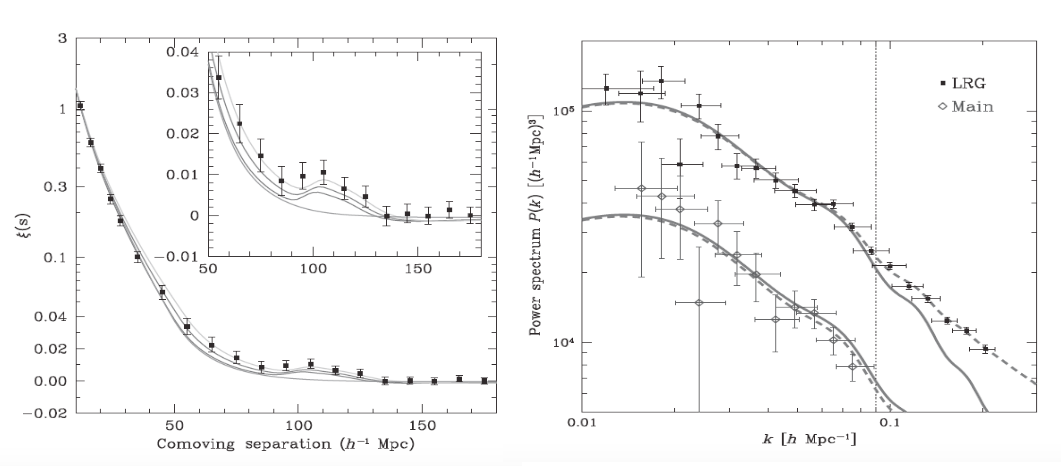
\includegraphics[width=0.95\textwidth]{Images/PS_CF.png}
       \caption{\small BAO peak in the correlation function in the left and the oscillations of BAO in the power spectrum in the right,
       (\cite{PLOT}).  
       The lower curve is the main SDSS sample and the upper one is the LGR sample, (\cite{PLOT2}). }
       \label{ps_cf}
 \end{figure}
%**********************************************************************************************************************

The isotropy of the universe is taken into account during the power spectrum calculation because an average is done over
all  possible orientations of the vector ${\mbox{\boldmath$\kappa$}}$, as it can be seen in the expression (\ref{pk}) . 


 Additionally it has been found that the initial power spectrum 
expected from inflation theories has the form $P(\kappa)= k^n$. If $n=1$ the power spectrum is called 
Harrison-Zeldovich which is commonly used. 


With the initial power spectrum it can be done an inverse fourier transform and this way creating the initial 
density field. 

\

It is necessary to consider that after the recombination epoch the density contrasts started growing in size 
causing a non linear growth to appear. This implies a change in the density field and likewise the power spectrum. 

\subsubsection*{ Baryonic acoustic oscillations }

Let us consider the epoch before recombination. The baryonic plasma (ionized protons and electrons) was coupled with radiation via 
Thomson scattering,  i.e., the electric field of photons accelerate charged particles making small density contrast to disperse. Nevertheless,
considering that dark matter do not interact with radiation, small dark matter density contrasts can form. Hence, the baryons are 
subject to two competing forces, radiation pressure and gravitation. Consider a particular dark matter density contrast that attract
nearby baryons, they start clustering around the dark matter forming a bigger density contrast. But, due to the pressure caused
by coupling, the outward force becomes bigger than gravity, making baryons to move outward as a sound wave. This oscillation 
of the baryonic plasma is known as baryonic acoustic oscillation (\cite{pilar}). 

\

When decoupling occurs and temperature drops, the force responsible for the expansion of the shell disappear, this is, 
the pressure caused by the coupling between baryons and radiation, leading baryons in the last position they were located. 
The scale of the baryonic acoustic oscillation is 
usually called the sound horizon and it can be computed as

\[  
s = \int_{z_{rec}}^{\infty} \f{c_s dz}{H(z)}
\]


where $c_s$ is the velocity of the propagation and $H(z)$ is the hubble param, (\cite{pilar}). 

Therefore, there is a spherical shell formed 
around the dark matter density contrast. Now, not only dark matter density contrast seed gravitational instability but 
the baryons on the shell. 

The structures continue to grow reaching non linear growth and wipe out the imprint lead by the baryonic acoustic
oscillations except for the bigger ones. The estimated size of the remaining BAO is $105$Mpc, causing that scale to 
be more likely to have galaxy formation activity. The reason this distribution is not observed at cosmological scales is because
of the amount of imprints, they smear out the preferred scale. Though, it is expected an enhancement in the two point
correlation at scales of the baryonic oscillations. As was seen before, there is a direct correspondence between the 
two point correlation and the power spectrum. Hence, a characteristic oscillation in the power spectrum caused by the imprint of BAO 
is naturally found. 	

 
%**********************************************************************************************************************
\begin{figure}[htbp]
       \centering
               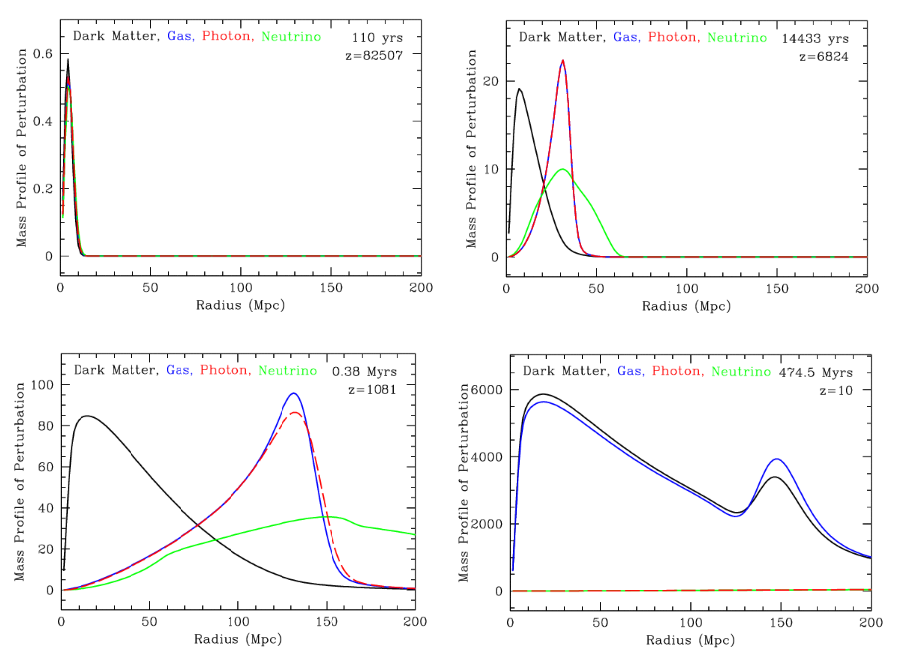
\includegraphics[width=1.0\textwidth]{Images/BAOS2.png}
       \caption{\small All the figures show the evolution of the radial mass profile of dark matter,  baryons, photons
       and neutrinos. First one: Initial perturbations of the four species. 
       Second one: the neutrinos do not interact and move away, 
       the plasma of baryons and radiation overdensity expands because of radiation pressure, the dark matter
       continues to fall in the perturbation. Third one: The temperature drops enought to lead to decoupling, 
      the baryons slows down until stopped, the radiation and neutrinos continue moving away. Fourth one:  
      The dark matter and baryons eventually get the same distribution because of the gravitational interaction, (\cite{10MPC}).}
       \label{DBM}
 \end{figure}
%**********************************************************************************************************************

Since baryonic acoustic oscillations are primarily a linear phenomenon, they are preserved in the power spectrum despite of 
the temporal evolution. Then,  BAO are used as an standard ruler, specifically for high redshift where other rulers tend to fail. 
This is commonly used for constraining dark matter models. 

\

Although, the nonlinear collapse change the shape and position of baryonic acoustic oscillations, broaden and shift the 
peak. This is clearly seen in the figure (\ref{peak}), the broadening of the peak initially shown as a very sharp causes 
a damping in the frequency in the power spectrum. It is expected that this effect that is going to be studied in this work, affects baryonic 
acoustic oscillations on scales around $\sim 10$Mpc, (\cite{10MPC}). 

The diffusion damping (silk damping)  also causes a reduction in size of density inequalities by the diffusion of photons from 
hot regions to colder ones during the epoch of recombination. 

%**********************************************************************************************************************
\begin{figure}[htbp]
       \centering
               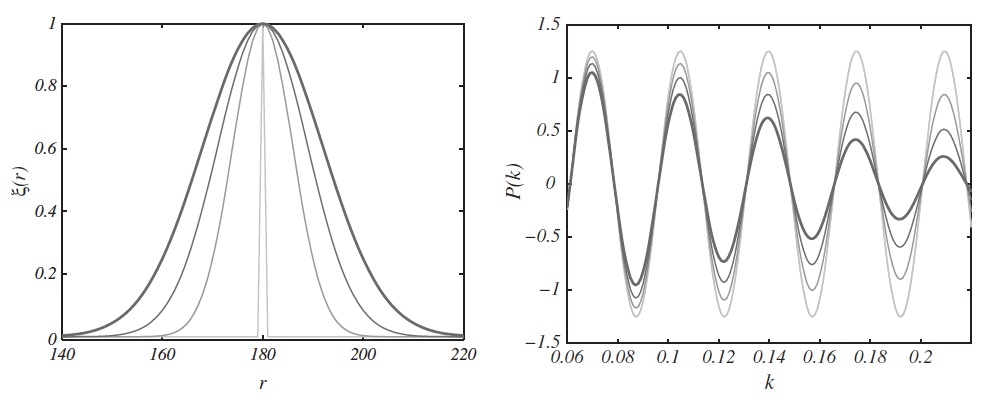
\includegraphics[width=0.9\textwidth]{Images/width.png}
       \caption{\small In the left the correlation function and the right the power spectrum. When the width of the peak is increased
       the acoustic oscillation obtained in the power spectrum is damped, \cite{pilar}.    }
       \label{peak}
 \end{figure}
%**********************************************************************************************************************


\subsubsection*{ Construction of the power spectrum }
\label{subsubsec:CPS}

Despite of the fact that there are several approaches to study the evolution of the universe, one commonly used is cosmological
simulations. But, how can a density field and also the power spectrum be calculated in such a case in order to find the baryonic
acoustic oscillations? 

\

There are various recipes to construct the density field from a discrete point distribution, 
including Nearest Grid Point (NGP), cloud in cell (CIC), triangular shaped cloud (TSC), Voronoi or
delaunay tessellations. 

Let us see in more detail CIC. It considers a regular grid but takes into account the contribution to a cell of particles that fall in and neighboring 
cells. Then, a particle contributes at most to eight masses of different cells. The constructed density field is finally 
given by the mass of every cell. 

\

With the density field constructed it is possible to find the power spectrum of the simulation. First, using the fast fourier transform (FFT)
a fourier transform of the density field is performed.  This leads to density contrasts in the fourier space. Finally, mean of the magnitude
squared of the contrast density is estimated by shells in the fourier space. 

\

Due to the discreteness of the system, there is an error in the power spectrum calculation,  shot noise. 
It is an effect caused by sample size, patterns can be erased if there is no enough particles to display 
all the information needed for certain study. 
It makes necessary to introduce an additional term in the power spectrum -$1/N$ where N is the number of particles. 

\

In addition to shot noise, alias effect makes necessary to introduce another correction to the power spectrum. The mass assignment in the 
construction of the density field is equivalent to make a convolution of the density field by a given assignment function $W(\textbf{r})$.
Now, FFT  of the density field is finite, then the series is truncated. This leads to possible important modes not to be included in the 
power spectrum. A possible correction proposed to this problem is included in \cite{alias}. 

\

Furthermore, because of the limited size, there is an error in the estimation of clustering at larger scales than the box or 
survey size. This can be solved partially having a lot realizations of the system.  

\subsubsection*{ Mass density reconstruction: Halo based method }
\label{subsubsec:HBM}


As was previously mentioned, it is essential a comparison between cosmological simulations and observations 
in the search of constraining the properties of baryonic acoustic oscillations. Now that it has been exposed the 
way to obtain them from a cosmological simulation, it is necessary to explain the way the power spectrum is going 
to be built from observations. First, for observations is enough to construct the density field of the survey and then apply
the same procedure to construct the power spectrum though some additional corrections could be considered. 

\

As can bee seen in figure (\ref{DBM}) there is a difference in the radial mass profile of DM and
baryons, this is, a difference in the distribution of DM and baryonic matter. Generally, this difference is measured 
through a bias factor but since dark matter can not be observed there are suppositions implied on these biases factors. 
The method that will be used in this project is exposed in \cite{HBM}, \cite{HBM01} and avoids using a bias factor explicitly in the estimation of 
dark matter distribution from observational data. This is achieved creating 
galaxy groups from observations and from them estimating the dark matter distribution. 
One of the benefits of the method besides that there is no bias assumption, it is that it is parameter free;  parameters such
as linking length, density threshold, among others. 

\ 

The method estimates the mass distribution as is explained below.  
Consider a typical distribution of a halo  $\eta (r,M)$ of mass $M$ in and around dark matter halos, 
where $r$ is distance from the center of the halo. This function can be found from simulations. 
And a known spatial coordinates and masses of a set of DM halos in the function $\Phi(\vec{r}_i,M_i)$, where $\vec{r}_i$ is 
the position of the halo $i$ of mass $M_i$ in a halo catalog taken for the reconstruction. 
Hence, the mass density distribution is given by the convolution of the typical 
distribution and the function $\Phi(\vec{r}_i,M_i)$

\[
\rho_i(\vec{r}_i,M_i) = \eta (r,M) \otimes  \Phi(\vec{r}_i,M_i)
\]

the total mass density due to all the set of halos can be expressed as 

\[
\rho = \hat{\Sigma} \rho_i(\vec{r}_i,M_i)
\]

where $\hat{\Sigma}$ is a sum for isolated halos, i.e., domains that do not overlap each other. If they do overlap
then $\hat{\Sigma}$ has to take into account the extension of their local domain and the environment. 

Using this method to perform the reconstruction of the density field,  it would be possible to construct the power spectrum
as was explained in the previous section. 


%==============================================================================
\section{Methodology}
%==============================================================================

The work consists in analysing the behaviour of BAO in different scenarios, then it is fundamental
to find a way to obtain the BAO either, from simulations or observations. For this reason, 
it becomes necessary to develop a numerical tool to find such BAO in any case. But in order to 
build such a tool it is obviously needed a physical model that can account for BAO. 
Using the numerical tool there are going to be done several realizations, this is done seeking to avoid errors
associated to cosmic variance. Finally after this is done, there is going to be an 
analysis and comparison of the BAO in simulation (theoretical model) against the BAO recovered from observations,
in order to find the arguments to answer the questions we formulated for the project.

\

A more detailed procedure is shown below.

\begin{itemize}

\item[-] \textbf{ Bibliographical review }
	
In this first stage we will look for books, reviews and papers related to the physics of 
BAO, the different ways to find BAO through the density field or correlation function, the 
power spectrum, power spectrum calculation and corrections associated. As well as a search 
through data base, specially to look for observational data  from the SDSS (DR-7 and DR-12) 
that are going to be used.

\item[-] \textbf{ Construction of models } 

Using the information collected in the bibliographical review
it will be chosen a model to estimate the density field of a numerical cosmological simulation,
the power spectrum and the corrections to take into account. Equally, for the observational
data collected is going to be used an specific model to construct the dark matter halos
from which  BAO are going to be found.

\item[-] \textbf{ Model implementation } 

In this section it will be coded the models proposed, i.e. ,
a model to obtain BAO from numerical cosmological simulations and BAO from observational data.  
The code will allow to make several numerical realizations of different numerical
simulations and compare them with the BAO obtained from observations. 

\item[-] \textbf{ Analysis and conclusions } 

It is necessary to analyse the results obtained in the 
previous sesion. One of the most important 
issue is to characterize the BAO through this results and show if there are changes in its properties  
with the cosmological scale, specifically if there is any possible change in the position or 
width of the BAO signal.  

\item[-] \textbf{ Thesis and paper } 

The results and conclusions will be written in  a master thesis and 
an article. 

\end{itemize}

%==============================================================================
\section{Expected Results}
%==============================================================================

The expected results when finishing the master studies are 

\begin{itemize}

\item[-] A set of tools to estimate the signal of BAO in numerical cosmological simulations, that also includes 
corrections to the power spectrum that possibly affect the BAO results. 

\item[-] Obtain BAO from observations, SDSS (DR-7 and DR-12), and conclude what changes appear 
in the width and position of the BAO with the structure scale. 

\item[-] Comparison between the results obtained with numerical cosmological simulations
and the BAO obtained from observations to determine in an optimal way the properties of the BAO.  

\item[-] Study the dependence of tracer bias on the BAO properties measured in the observations. 

\item[-] A master thesis with the results obtained. 

\item[-] A submitted article with the results obtained.  

\end{itemize}

%==============================================================================
\section{Scientific Impact}
%==============================================================================


A very active investigation field is dark energy (DE), it is about $70\%$ of the content of energy and
matter of the universe but it has not been clearly understood nowadays. A equation of state (EOS) of the dark
energy is then a relevant issue to be studied and in general it depends on the redshift, i.e., $w(z)$. Then
it becomes necessary to have standard rulers for different stages, including high redshifts. Therefore, the 
BAO allows to get tight constraints on the parameters of the DE EOS. 

Moreover, the BAO signal provides a key understanding of the accelerated expansion of the universe since
it provides a way to obtain the hubble parameter and the angular size of objects depending on redshift.  

\

Hence, the relevance of this work is study the properties of the BAO and this way to provide a better understanding
of their behaviour, specifically to observe what are the changes in their position and width due to the scale of the 
tracer halo population. This will possibly allow to include more corrections to the BAO signal and 
get a more profound insight in the physics of BAO. 


%==============================================================================
\section{Schedule}
%==============================================================================
Next it is shown a table with the proposed activities scheduled for each term.

\begin{table}[h]
\begin{flushleft}
\begin{center}
  \begin{tabular}{l  c c c c } \hline\hline
	\centering\textbf{Goals} & \textbf{Semester I} & \textbf{Semester II} & 
	\textbf{Semester III} & \textbf{Semester IV} \\ \hline\hline
	
	 Bibliographical review & X & X & & \\
	 Construction of models & X & X & & \\
	 Model implementation &  & X & X & \\
	 Analysis and conclusions &  &  & X & X \\
	 Thesis and paper &  &  &  & X \\
	\hline\hline
  \end{tabular}  
  \caption{ Terms range from 2015-02 for term I, up to 2017-01 for term IV.}
\end{center}
\end{flushleft}
\end{table}


%==============================================================================
\bibliographystyle{latex/mn2e}
%\bibliographystyle{acm}
\renewcommand{\bibname}{11\ \ \ \ Bibliography}
\small
\bibliography{References.bib}
%==============================================================================

\end{document}